\section{SIMULAÇÃO DE SISTEMAS DINÂMICOS}\label{sec:2gym-gymependinv}

Foi mencionada a importância de se analisar o problema em que se deseja aplicar a programação genética. Essa análise permite a escolha da função de avaliação, das variáveis terminais e dos operadores. Ao estudar o pêndulo invertido, é possível verificar como um sistema dinâmico pode ser abordado com a PG.

\subsection{PÊNDULO INVERTIDO}\label{ssec:2gym-sistdin}

O pêndulo invertido pode ser considerado um dos sistemas robóticos mais simples, composto apenas por um corpo rígido e um ponto de rotação. Apesar da sua simplicidade, muitas técnicas padrões, derivadas da teoria de controle, são ineficientes e, por isso, o sistema tem importância considerável na área de controle não-linear~\cite{olfa13PendInv}.

Existem diversas variações desse sistema~\cite{wang11PidIp}. O caso abordado neste trabalho trata de um bastão apoiado sobre um veículo que se movimenta com apenas um grau de liberdade, sendo a sua posição dada pela variável $\mathbf{s}$. O ângulo $\mathbf{\theta}$ representa a inclinação do bastão em relação a uma reta normal à superfície. O controle deve ser exercido por uma força $\mathbf{F}$, aplicada paralelamente à superfície, em qualquer sentido, com a finalidade de manter $\theta\approx 0^{\circ}$.

\begin{figure}[!h]
\centering
\includegraphics[width=0.6\linewidth]{02_desenvolvimento/02_PInv_Fig_CartPole.png}
\caption{Sistema do pêndulo invertido.}\label{fig:2gym-cartpole}
\end{figure}

O sistema de equações diferenciais que modela a dinâmica do problema é descrito na Equação \ref{eq:2gym-sisteq}.

\begin{align}\label{eq:2gym-sisteq}
\ddot{\theta} &= \dfrac{g\sin\theta+\cos\theta\left[
\dfrac{-F-m_cl\dot{\theta}^2\sin\theta+\mu_c\sign{(\dot s)}}{m_c+m_b}\right] - \dfrac{\mu_p\theta}{m_bl}}
{l
\left[\dfrac{4}{3} - \dfrac{m_b\cos^2\theta}{m_c+m_b}
\right]}\nonumber\\\\
\ddot{s} &= \dfrac {F+m_bl\left[ \dot{\theta}^2\sin\theta-\ddot\theta\cos\theta \right]
-\mu_c\sign(\dot s)}
{m_c+m_b}\nonumber
\end{align}

Onde:

\begin{itemize}[label=\raisebox{0.25ex}{\tiny$\bullet$}]
\item $g$ = -9,8 \si{m/s^2}, aceleração causada pela gravidade;
\item $m_c$ = 1,0 \si{kg}, massa do carro;
\item $m_b$ = 0,1 \si{kg}, massa do bastão;
\item $l$ = 0,5 \si{m}, metade do comprimento do bastão;
\item $\mu_c$ = 0,0005, coeficiente de atrito do carro na superfície;
\item $\mu_p$ = 0,000002, coeficiente de atrito do bastão no carro;
\item $F$ = $\pm$10,0 \si{N}, força aplicada no centro de massa do carro.
\end{itemize}

Barto et al.~\cite{barto83CartPole} utilizam o subscrito $t$ (omitido neste trabalho) para algumas variáveis, com a finalidade de explicitar a dependência do tempo discreto. A Equação \ref{eq:2gym-sisteq} serviu de base para a implementação do ambiente simulado na biblioteca \textit{Gym}~\cite{gymCartPole}.

\subsection{BIBLIOTECA ``OPENAI GYM’’}\label{ssec:2gym-openaigym}

Antes de discutir a implementação do sistema na biblioteca \textit{Gym}, é feita uma análise das suas principais funcionalidades. \textit{Gym} é uma biblioteca voltada principalmente para o teste de algoritmos de aprendizagem por reforço. Frequentemente, os ambientes de aprendizado para esses algoritmos são descritos através de \textit{processos de decisão Markovianos}.

A principal ideia dos sistemas Markovianos é a interação de um \textit{agente} com um \textit{ambiente} externo, através de ações, estados e recompensas, denotados por $A_t$, $S_t$ e $R_t$, respectivamente. A cada passo de tempo, o ambiente fornece ao agente o seu estado atual ($S_t$) e uma recompensa ($R_t$). Uma ação ($A_t$), gerada pelo agente, influenciará o sistema dinâmico no próximo instante. O objetivo do agente é maximizar a expectativa de recompensa acumulada ao longo do tempo, através de suas ações. Este processo é descrito graficamente na Figura \ref{fig:2gym-mdp}.

\begin{figure}[!h]
\centering
\includegraphics[width=0.8\linewidth]{02_desenvolvimento/02_PInv_Fig_Mdp.png}
\captionsource{Processo de decisão de Markov.}{Adaptado de~\cite{sutton18bookRl}.}
\label{fig:2gym-mdp}
\end{figure}

%Para processos Markovianos, um estado $S_t$ caracteriza completamente a dinâmica de um sistema, no instante $t$. Isto significa que para ambientes estocásticos Markovianos, dado um estado $S_t$ e uma ação $A_t$, sabemos a probabilidade associada a cada possível próximo estado, $S_{t+1}$ e recompensa futura $R_{t+1}$. Não há probabilidades associadas ao sistema do pêndulo invertido, logo, para o nosso problema, se há um estado Markoviano $S_t$ observável, saberemos com precisão qual será o próximo estado do sistema e a recompensa futura recebida pelo agente.

Para processos de decisão Markovianos, $R_t$ e $S_t$ são variáveis aleatórias com distribuições de probabilidade que dependem apenas do estado e ação anteriores, $S_{t-1}$ e $A_{t-1}$, respectivamente. Para sistemas determinísticos, como os que são abordados neste trabalho, há um mapeamento $S_t,\,A_t \to S_{t+1}$.

As simulações da biblioteca Gym são baseadas em processos de decisão Markovianos. Portanto, a cada iteração existe uma variável acessível ao agente, que indica o estado atual do ambiente e sua recompensa, $S_t$ e $R_t$, respectivamente. O agente será a máquina que aprende com a experiência, mais especificamente, com informações de estados e recompensas obtidas ao longo do tempo.

% Além disso, vimos que o agente influencia o sistema através de ações $A_t$, cuja implementação também é proporcionada pela biblioteca.

%Estados Markovianos descrevem completamente o próximo estado do ambiente. Por esse motivo, $S_t$ deve conter informações suficientes para que possamos prever o próximo estado. Essa restrição imposta aos estados explica o motivo da observação fornecida ao agente pela biblioteca. Mais especificamente, para o problema do pêndulo invertido, a observação fornecida ao agente inclui as variáveis de estado:

Estados Markovianos devem conter informações suficientes para que, dadas uma ação e uma observação do estado atual, seja possível prever o próximo estado. Desta forma, fica claro que a observação fornecida deve conter dados sobre as variáveis de estado do sistema.

%pois essa informação aliada à entrada gerada pelo agente (força $\mathbf{F}$) é suficiente para indicar o próximo estado.

\begin{table}[!htb]
\centering
\caption{Variáveis de estado fornecidas como observação do estado atual ($S_t)$).}
\label{tab:2gym-observacao}
\begin{tabular}{l|l|l|l} \toprule
{Variável} & {Significado} & {Valor Mínimo} & {Valor Máximo}\\ \midrule
{$s$} & {Posição do carro} & {$-4.8$} & {$4.8$} \\
{$\dot{s}$} & {Velocidade do carro} & {$-\infty$} & {$\infty$} \\
{$\theta$} & {Ângulo do bastão} &{$\SI{-24}{\degree}$} & {$\SI{24}{\degree}$} \\
{$\dot\theta$} & {Velocidade angular do bastão} & {$-\infty$} & {$\infty$}
\\ \bottomrule
\end{tabular}
\end{table}

A simulação ocorre em episódios de duração limitada: o término acontece quando as variáveis de estado ou o tempo decorrido excedem um certo valor, conforme exemplifica a Tabela 1.

A implementação de recompensas ($R_t$) no ambiente do pêndulo invertido é simples: a cada instante de tempo, o agente recebe $1$ de recompensa. Controladores com baixo desempenho irão forçar o término do episódio rapidamente, recebendo pouca recompensa. 

Os componentes da simulação estão implementados na linguagem de programação \textit{Python}, utilizando classes e categorias de dados específicos.

\begin{figure}[H]
\centering
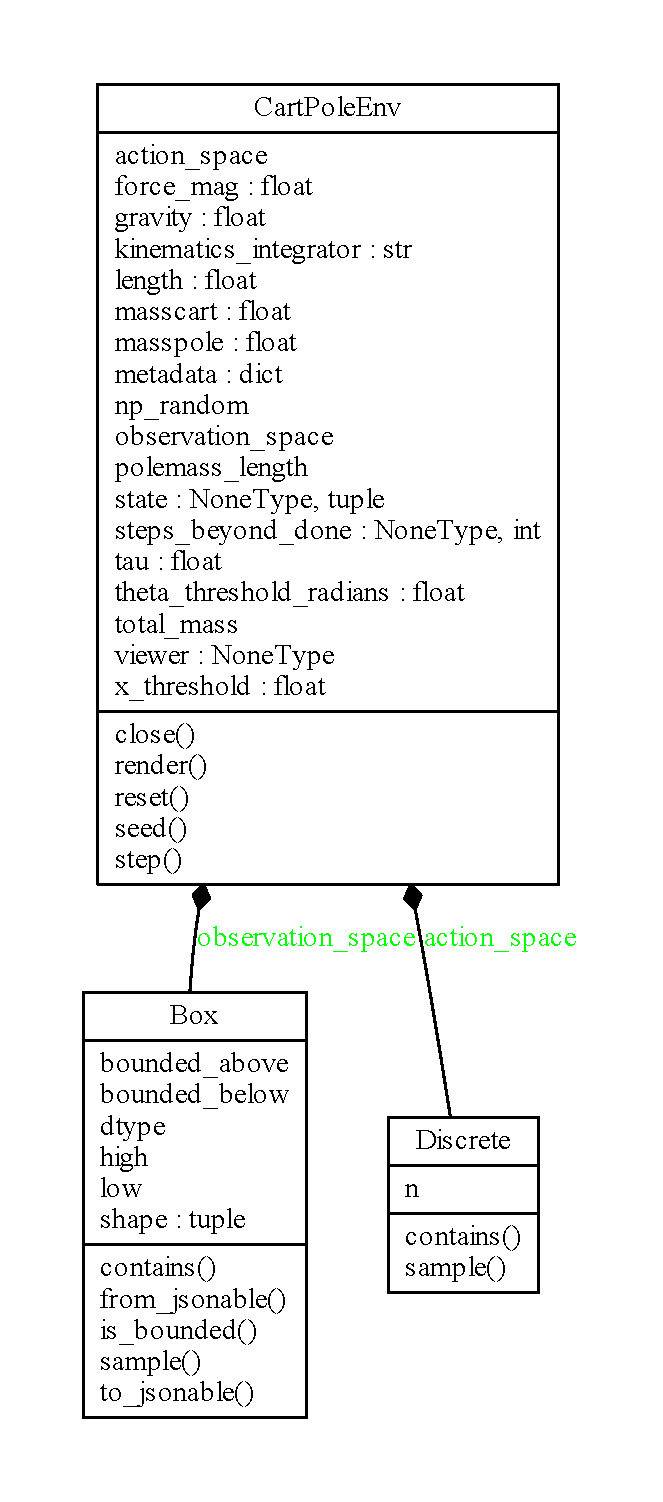
\includegraphics[width=0.5\linewidth]{02_desenvolvimento/02_PInv_Fig_ClassUML.pdf}
\caption{Diagrama de classes para o ambiente de simulação do pêndulo invertido, gerado com o utilitário \textit{pyreverse}.}\label{fig:2gym-umlclasse}
\end{figure}

Na Figura \ref{fig:2gym-umlclasse}, é possível verificar que os objetos \textit{observation\_space} e \textit{action\_space} pertencem às classes \textit{Box} e \textit{Discrete}, respectivamente, e compõem o ambiente de simulação. Essas classes determinam quais são as observações e ações possíveis na simulação, isto é, impõe restrições às ações que o agente pode tomar e à observação recebida. Na simulação do pêndulo invertido, as ações estão restritas aos valores inteiros $0$ e $1$, por exemplo, indicando a aplicação da força para a esquerda ou para a direita. Os métodos disponíveis são utilizados para realizar a interação do agente com o ambiente. As principais funções existentes são detalhadas a seguir:

\begin{enumerate}[label=\alph*)]
\item \textbf{\underline{make(\textit{nome})}}:
\begin{itemize}[label=\raisebox{0.25ex}{\tiny$\bullet$}]
\item \textbf{Descrição}: cria um objeto em que ocorre a simulação.
\item \textbf{Argumento}: (\textit{String}) nome do ambiente de simulação. Ex: 'CartPole-v1'
\item \textbf{Retorno}: (\textit{Env}) Ambiente de simulação.
\end{itemize}
\item \textbf{\underline{reset(\textit{ambiente})}}:
\begin{itemize}[label=\raisebox{0.25ex}{\tiny$\bullet$}]
\item \textbf{Descrição}: inicia um episódio de simulação, com valores iniciais aleatórios dentro de uma faixa específica.
\item \textbf{Argumento}: (\textit{Env}) o objeto (ambiente de simulação) que será inicializado.
\item \textbf{Retorno}: (\textit{Box}) observação (objeto) que contém o valor das variáveis de estado.
\end{itemize}
\item \textbf{\underline{step(\textit{ambiente}, \textit{ação})}}:
\begin{itemize}[label=\raisebox{0.25ex}{\tiny$\bullet$}]
\item \textbf{Descrição}: realiza a \textit{ação} no sistema.
\item \textbf{Argumento}: (\textit{Env}, \textit{Int}) objeto com o ambiente de simulação e ação discreta do agente.
\item \textbf{Retorno}: (Tupla) uma tupla que contém: observação (após a ação do agente), recompensa, indicação de término do episódio e informações adicionais.
\end{itemize}
\item \textbf{\underline{render(\textit{ambiente}, \textit{modo})}}:
\begin{itemize}[label=\raisebox{0.25ex}{\tiny$\bullet$}]
\item \textbf{Descrição}: renderiza o ambiente de simulação.
\item \textbf{Argumento}: (\textit{Env, String}) ambiente a ser simulado e o modo de exibição.
\item \textbf{Retorno}: objeto de renderização.
\end{itemize}
\end{enumerate}

As funções descritas são métodos que atuam no ambiente de simulação. A utilização dessas funções pode ser exemplificada no fluxograma da Figura \ref{fig:2gym-ciclogym}.

\begin{figure}[H]
\centering
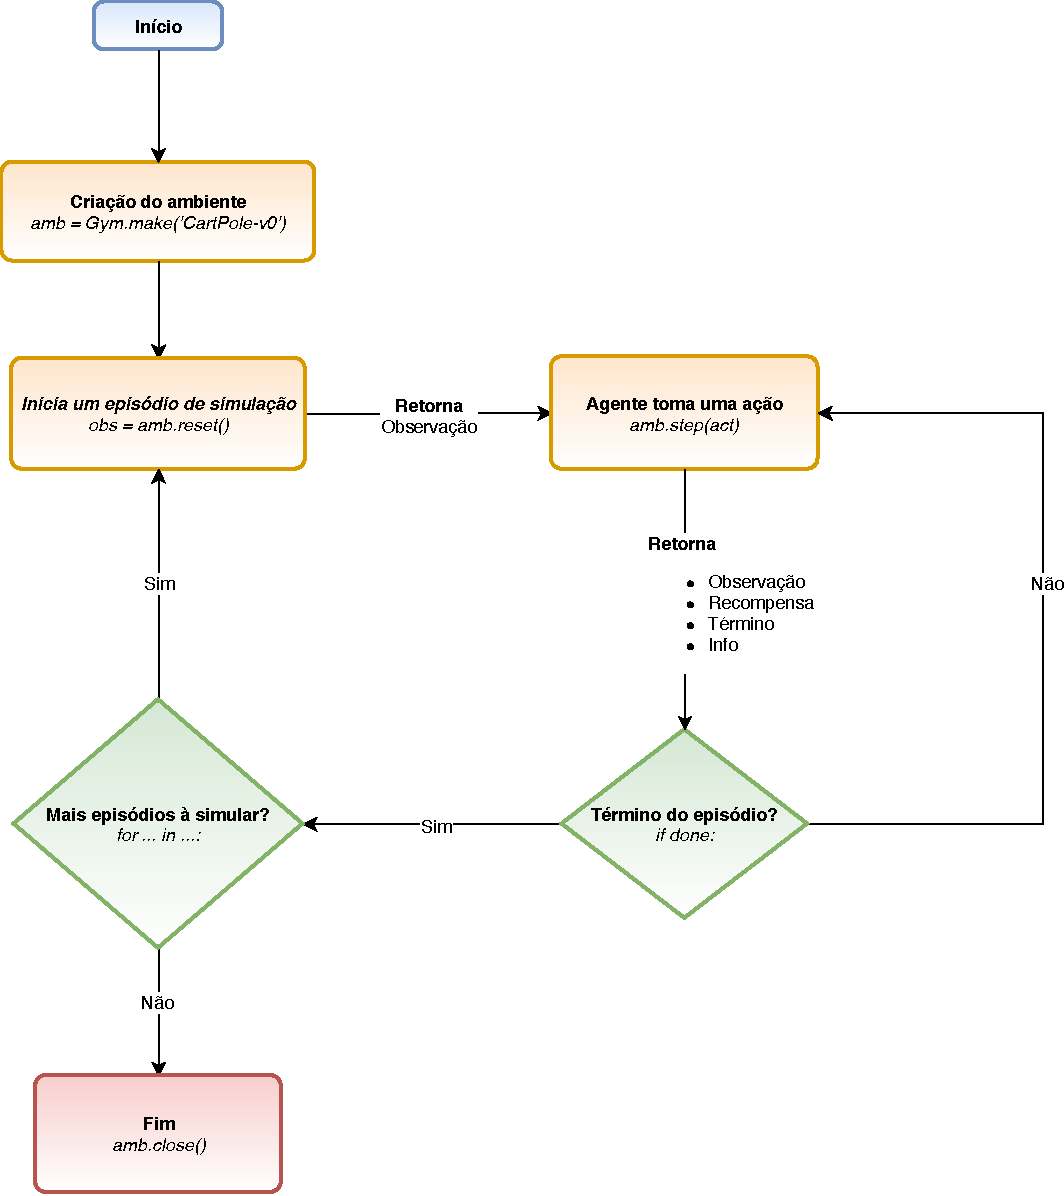
\includegraphics[width=1\linewidth]{02_desenvolvimento/02_PInv_Fig_CicloGym.pdf}
\caption{Forma geral de um algoritmo para realização de uma simulação no \textit{OpenAi Gym}.}\label{fig:2gym-ciclogym}
\end{figure}

É realizado, a seguir, uma análise breve de cada objeto da interação demonstrada na Figura \ref{fig:2gym-ciclogym}, com o objetivo de facilitar a criação do algoritmo.

O principal objeto é o retornado pela função \textit{step}. Trata-se de uma tupla de quatro objetos, os quais o agente utilizará para obter informações sobre o sistema, quais sejam:

\begin{itemize}[label=\raisebox{0.25ex}{\tiny$\bullet$}]
\item \textit{Observação}: lista indexável (Figura \ref{fig:2gym-observacao}) que contém o valor das variáveis de estado do sistema logo após a \textit{ação} do agente.
\begin{figure}[H]
\centering
\includegraphics[width=0.6\linewidth]{02_desenvolvimento/02_PInv_Fig_Observacao.png}
\caption{\textit{Box} é uma classe que permite a criação de conjuntos multidimensionais, no ambiente do pêndulo invertido é apenas uma lista (unidimensional).}\label{fig:2gym-observacao}
\end{figure}
\item \textit{Recompensa}: valor retornado pelo sistema após ter sofrido uma \textit{ação} do agente. Pode apresentar os valores $0$ ou $1$, para o ambiente do pêndulo invertido (Figura \ref{fig:2gym-recompensa}).
\begin{figure}[!h]
\centering
\includegraphics[width=0.15\linewidth]{02_desenvolvimento/02_PInv_Fig_Recompensa.png}
\caption{Recompensa recebida pelo agente.}\label{fig:2gym-recompensa}
\end{figure}
\item \textit{Término}: valor lógico (Figura \ref{fig:2gym-termino}) que indica se o episódio de simulação terminou ou não, de acordo com os critérios estabelecidos.
\begin{figure}[!h]
\centering
\includegraphics[width=0.10\linewidth]{02_desenvolvimento/02_PInv_Fig_Termino.png}
\caption{Valor lógico que indica se o episódio terminou ou não.}\label{fig:2gym-termino}
\end{figure}
\item \textit{Info}: fornece informações adicionais sobre a simulação ao programador. Geralmente, é utilizada para \textit{debugging}.
\end{itemize}

Ao longo deste capítulo foi possível estudar a implementação da simulação de sistemas dinâmicos na biblioteca \textit{Gym}. Esta é uma etapa essencial para verificar o desempenho das soluções encontradas ao longo da execução do algoritmo. O próximo capítulo aborda outros aspectos da programação genética, através da biblioteca DEAP.